\documentclass{pset}

\renewcommand{\hmwkTitle}{6th\ hw}
\renewcommand{\hmwkDueDate}{February 12, 2014}
\renewcommand{\hmwkClass}{Measure Theory}
\renewcommand{\hmwkClassTime}{Chapter 7}
\renewcommand{\hmwkAuthorName}{}

%
% Title Page
%

\title{
    \vspace{2in}
    \textmd{\textbf{\hmwkClass:\ \hmwkTitle}}\\
    \normalsize\vspace{0.1in}\small{Due\ on\ \hmwkDueDate\ at 3:10pm}\\
    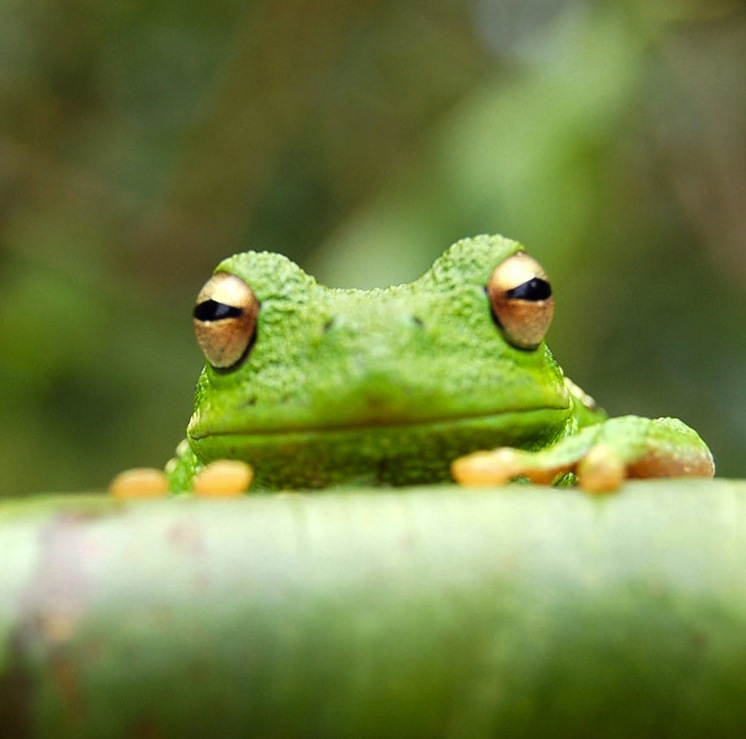
\includegraphics[scale=0.2]{frog} \\
    \vspace{0.1in}\large{\textit{\hmwkClassTime}}
    \vspace{3in}
}

\author{\hmwkAuthorName}
\date{}

\renewcommand{\part}[1]{\textbf{\large Part \Alph{partCounter}}\stepcounter{partCounter}\\}
\newcommand{\ev}{\operatorname{ev}}

\begin{document}
first we note that $\{A_i^c\}_0^\i$ are also indepandent since
\[P(A_i)=P(A_i\cap A_j)+P(A_i \cap A_j^c) = P(A_i)P(A_j)+P(A_i\cap A_j^c)\]
hence for all $i\neq j$
\[P(A_i\cap A_j^c)=P(A_i)P(A_j^c)\]
and by that same argument we can see that
\[P(A_i^c\cap A_j^c)=P(A_i^c)P(A_j^c)\]
moreover,
\begin{align*}
P\Bigl(\bigcap_{k=0}^\i\bigcup_{i=k}^\i A_i\Bigr) &= \lim_{k\to\i}P\Bigl(\bigcup_{i=k}^\i A_i\Bigr) \\
&= \lim_{k\to\i}1-P\biggl(\Bigl(\bigcup_{i=k}^\i A_i\Bigr)^c\biggr) \\
&= \lim_{k\to\i}1-P\Bigl(\bigcap_{i=k}^\i A_i^c\Bigr) \\
&= \lim_{k\to\i}1-\prod_{i=k}^\i P(A_i^c)
\end{align*}
\end{document}